% DMA Session 9: JOINs
% 180-Minuten-Block (Vorlesung + Übung interwoven)

\documentclass[usenames,dvipsnames,10pt,aspectratio=169]{beamer}
\usepackage[T1]{fontenc}
\usepackage[utf8]{inputenc}
\usepackage{verbatim}

\usetheme{ims}

\usepackage{booktabs}
\usepackage{multicol}
\usepackage{listings}
\usepackage[table]{xcolor}
\usepackage{graphicx}
\usepackage{tikz}
\usetikzlibrary{shapes.geometric, arrows.meta, positioning, calc, fit, backgrounds, matrix}
\usepackage{pifont}

% TikZ styles
\tikzset{
    tablebox/.style={rectangle, draw=IMSBlue, fill=IMSBlue!5, thick,
        minimum width=4cm, minimum height=0.8cm, font=\ttfamily\small},
    tableheader/.style={rectangle, draw=IMSBlue, fill=IMSBlue!20, thick,
        minimum width=4cm, minimum height=0.8cm, font=\ttfamily\small\bfseries},
    roadmapbox/.style={rectangle, rounded corners, minimum width=2.5cm, minimum height=0.8cm,
        text centered, draw=IMSBlue, fill=IMSBlue!10, font=\small\bfseries},
    roadmaparrow/.style={-{Stealth[length=3mm]}, thick, IMSBlue},
    joinbox/.style={rectangle, rounded corners, minimum width=2cm, minimum height=1.5cm,
        text centered, draw=IMSBlue, thick, font=\bfseries},
    vennset/.style={circle, draw=IMSBlue, thick, minimum size=2.5cm, fill opacity=0.3},
    sqlbox/.style={rectangle, rounded corners, draw=IMSOrange, fill=IMSOrange!10,
        minimum width=2cm, minimum height=0.6cm, font=\small},
    sqlarrow/.style={-{Stealth[length=2.5mm]}, thick, IMSOrange},
    graphnode/.style={circle, draw=IMSBlue, fill=IMSBlue!20, thick, minimum size=0.8cm, font=\small\bfseries},
    graphedge/.style={-{Stealth[length=2.5mm]}, thick, gray},
    quizbox/.style={rectangle, rounded corners, draw=IMSBlue, fill=IMSBlue!5,
        minimum width=8cm, minimum height=1cm, font=\normalsize},
}

% SQL Listing Style
\lstdefinestyle{sql}{
    language=SQL,
    basicstyle=\ttfamily\footnotesize,
    keywordstyle=\color{IMSBlue}\bfseries,
    stringstyle=\color{IMSOrange},
    commentstyle=\color{gray}\itshape,
    showstringspaces=false,
    breaklines=true,
    frame=single,
    backgroundcolor=\color{gray!10},
    morekeywords={SERIAL, BOOLEAN, TEXT, REFERENCES, CONSTRAINT, CASCADE, RESTRICT, PRIMARY, FOREIGN, KEY, UNIQUE, CHECK, DEFAULT, AUTO_INCREMENT, INT, VARCHAR, DATE, DECIMAL, NOT, NULL, INNER, LEFT, RIGHT, FULL, OUTER, CROSS, USING, NATURAL},
    literate={ü}{{\"u}}1 {ä}{{\"a}}1 {ö}{{\"o}}1 {Ü}{{\"U}}1 {Ä}{{\"A}}1 {Ö}{{\"O}}1 {ß}{{\ss}}1
}

\lstset{style=sql}

\newcommand{\cmark}{\textcolor{green!70!black}{\ding{51}}}
\newcommand{\xmark}{\textcolor{red}{\ding{55}}}
\newcommand{\pk}[1]{\underline{\texttt{#1}}}
\newcommand{\fk}[1]{\texttt{\textcolor{IMSOrange}{#1}}}

% ===== CLICKABLE AGENDA WITH PROGRESS INDICATOR =====
\usepackage{hyperref}
\hypersetup{colorlinks=false, pdfborder={0 0 0}}

% Phase counter for progress tracking
\newcounter{currentphase}
\setcounter{currentphase}{0}

% Clickable agenda item
\newcommand{\agendaitem}[3]{%
    \ifnum#1=#2
        \textcolor{IMSOrange}{$\blacktriangleright$ \textbf{\hyperlink{phase#2}{#3}}}%
    \else
        \textcolor{gray!70}{\phantom{$\blacktriangleright$} \hyperlink{phase#2}{#3}}%
    \fi\\[0.3em]%
}

% Progress dots for footline (clickable)
\newcommand{\progressdots}{%
    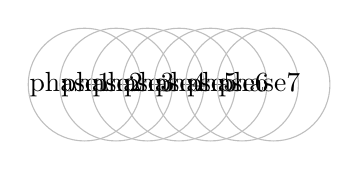
\begin{tikzpicture}[baseline=-0.5ex]
        \foreach \i in {1,...,7} {
            \ifnum\value{currentphase}=\i
                \node[circle, fill=IMSOrange, minimum size=0.24cm, inner sep=0pt] at (\i*0.4,0) {\hyperlink{phase\i}{\phantom{oo}}};
            \else
                \ifnum\value{currentphase}>\i
                    \node[circle, fill=IMSBlue!60, minimum size=0.2cm, inner sep=0pt] at (\i*0.4,0) {\hyperlink{phase\i}{\phantom{oo}}};
                \else
                    \node[circle, draw=gray!50, minimum size=0.2cm, inner sep=0pt] at (\i*0.4,0) {\hyperlink{phase\i}{\phantom{oo}}};
                \fi
            \fi
        }
    \end{tikzpicture}%
}

% Add progress indicator to footline
\setbeamertemplate{footline}{%
    \leavevmode%
    \hbox{%
        \begin{beamercolorbox}[wd=.33\paperwidth,ht=2.5ex,dp=1ex,left]{author in head/foot}%
            \usebeamerfont{author in head/foot}\hspace*{2ex}\insertshortauthor
        \end{beamercolorbox}%
        \begin{beamercolorbox}[wd=.34\paperwidth,ht=2.5ex,dp=1ex,center]{title in head/foot}%
            \progressdots
        \end{beamercolorbox}%
        \begin{beamercolorbox}[wd=.33\paperwidth,ht=2.5ex,dp=1ex,right]{date in head/foot}%
            \usebeamerfont{date in head/foot}\insertframenumber{} / \inserttotalframenumber\hspace*{2ex}
        \end{beamercolorbox}%
    }%
    \vskip0pt%
}

% Show agenda (with hyperlink target)
\newcommand{\showagenda}[1]{%
    \setcounter{currentphase}{#1}%
    \hypertarget{phase#1}{}%
    \begin{frame}{Agenda}
    \vfill
    \begin{center}
    \begin{minipage}{0.7\textwidth}
    \large
    \agendaitem{#1}{1}{1 ~ Rückblick \& Motivation}
    \agendaitem{#1}{2}{2 ~ INNER JOIN}
    \agendaitem{#1}{3}{3 ~ LEFT \& RIGHT JOIN}
    \agendaitem{#1}{4}{4 ~ Self-Joins}
    \agendaitem{#1}{5}{5 ~ Exkurs: Graphen in SQL}
    \agendaitem{#1}{6}{6 ~ Join-Performance}
    \agendaitem{#1}{7}{7 ~ Zusammenfassung}
    \end{minipage}
    \end{center}
    \vfill
    \end{frame}
}

%%%%%%%%%%%%%%%%%%%%%%%%%%%%%%%%%%%%%%%%%%%%%%%%%%%%%%%%%%%%%%%%%%%%%%%%%%%%%%%%%%%%%
\title[DMA 09]{Datenmanagement \& -analyse}
\subtitle{Vorlesung 9: JOINs}
\author{Prof. Dr. Christoph M. Flath}
\institute{Lehrstuhl für Wirtschaftsinformatik und Business Analytics\\Julius-Maximilians-Universität Würzburg}
\date{Sommersemester 2026}
%%%%%%%%%%%%%%%%%%%%%%%%%%%%%%%%%%%%%%%%%%%%%%%%%%%%%%%%%%%%%%%%%%%%%%%%%%%%%%%%%%%%%

\begin{document}

% ===== TITLE =====
\begin{frame}[plain]
    \titlepage
\end{frame}

% ===== PHASE 1: Rückblick & Motivation =====
\showagenda{1}

\begin{frame}{Rückblick: Der Weg zu normalisierten Daten}
\begin{center}
\begin{tikzpicture}[node distance=1.5cm]
    \node[roadmapbox] (real) {Reale Welt};
    \node[roadmapbox, right=of real, fill=green!10, draw=green!50!black] (er) {ER-Modell};
    \node[roadmapbox, right=of er, fill=green!10, draw=green!50!black] (rel) {Rel. Schema};
    \node[roadmapbox, right=of rel, fill=green!10, draw=green!50!black] (norm) {Normalisierung};
    \node[roadmapbox, right=of norm, fill=IMSOrange!20, draw=IMSOrange] (join) {JOINs};

    \draw[roadmaparrow] (real) -- (er) node[midway, above, font=\footnotesize] {\cmark};
    \draw[roadmaparrow] (er) -- (rel) node[midway, above, font=\footnotesize] {\cmark};
    \draw[roadmaparrow] (rel) -- (norm) node[midway, above, font=\footnotesize] {\cmark};
    \draw[roadmaparrow, IMSOrange, thick] (norm) -- (join) node[midway, above, font=\footnotesize] {Heute!};
\end{tikzpicture}
\end{center}

\vspace{1em}
\textbf{Letzte Session:}
\begin{itemize}
    \item Funktionale Abhängigkeiten
    \item Normalformen (1NF, 2NF, 3NF)
    \item Zerlegung in redundanzfreie Tabellen
\end{itemize}

\textbf{Diese Session:}
\begin{itemize}
    \item Wie fügen wir die Daten wieder zusammen?
    \item \textbf{JOINs} -- das Gegenstück zur Normalisierung!
\end{itemize}
\end{frame}

\begin{frame}{Motivation: Warum JOINs?}
\begin{columns}[T]
\column{0.5\textwidth}
\textbf{Nach der Normalisierung:}
\begin{itemize}
    \item Daten sind aufgeteilt
    \item Keine Redundanz
    \item Aber: Zusammenhänge verteilt!
\end{itemize}

\vspace{1em}
\textbf{Problem:}\\
``Welcher Spieler spielt für welchen Verein?''

\vspace{0.5em}
$\rightarrow$ Information in \textbf{zwei Tabellen}!

\column{0.5\textwidth}
\begin{center}
\begin{tikzpicture}[scale=0.85]
    \node[roadmapbox, minimum width=3cm] (spieler) at (0,2) {Spieler};
    \node[roadmapbox, minimum width=3cm] (vereine) at (0,0) {Vereine};
    \node[roadmapbox, minimum width=4cm, fill=IMSOrange!20, draw=IMSOrange] (ergebnis) at (0,-2) {Spieler + Verein?};

    \draw[roadmaparrow] (spieler.south) -- (ergebnis.north west);
    \draw[roadmaparrow] (vereine.south) -- (ergebnis.north east);
    \node[font=\large\bfseries, IMSOrange] at (1.5,-1) {JOIN};
\end{tikzpicture}
\end{center}
\end{columns}

\vspace{1em}
\begin{alertblock}{Kernidee}
\textbf{JOIN} = Verknüpfung von Zeilen aus verschiedenen Tabellen anhand einer gemeinsamen Bedingung.
\end{alertblock}
\end{frame}

\begin{frame}{Unser Beispiel-Schema}
\textbf{Normalisierte Bundesliga-Datenbank:}

\vspace{1em}
\begin{center}
\begin{tikzpicture}[scale=0.9, every node/.style={scale=0.9}]
    % Tables
    \node[rectangle, draw=IMSBlue, fill=IMSBlue!10, thick, minimum width=5cm, minimum height=1.5cm, align=center] (spieler) at (-4,0) {
        \textbf{Spieler}\\[0.3em]
        \pk{Spieler\_ID}, Name, Position, \fk{Verein\_ID}
    };

    \node[rectangle, draw=IMSBlue, fill=IMSBlue!10, thick, minimum width=5cm, minimum height=1.5cm, align=center] (vereine) at (4,0) {
        \textbf{Vereine}\\[0.3em]
        \pk{Verein\_ID}, Name, Stadt, Stadion
    };

    \node[rectangle, draw=IMSBlue, fill=IMSBlue!10, thick, minimum width=6cm, minimum height=1.5cm, align=center] (spiele) at (0,-3) {
        \textbf{Spiele}\\[0.3em]
        \pk{Spiel\_ID}, \fk{Heim\_ID}, \fk{Gast\_ID}, Datum, Heim\_Tore, Gast\_Tore
    };

    % Relationships
    \draw[-{Stealth}, thick, IMSOrange] (spieler.east) -- (vereine.west) node[midway, above] {Verein\_ID};
    \draw[-{Stealth}, thick, IMSOrange] (spiele.north west) -- (vereine.south west) node[midway, left, font=\footnotesize] {Heim\_ID};
    \draw[-{Stealth}, thick, IMSOrange] (spiele.north east) -- (vereine.south east) node[midway, right, font=\footnotesize] {Gast\_ID};
\end{tikzpicture}
\end{center}

\vspace{1em}
\textbf{Fragen, die JOINs beantworten:}
\begin{itemize}
    \item Welche Spieler spielen für Bayern München?
    \item In welchen Stadien fanden Spiele statt?
    \item Welche Vereine haben noch keine Spieler?
\end{itemize}
\end{frame}

\begin{frame}{Beispieldaten}
\begin{columns}[T]
\column{0.45\textwidth}
\textbf{Spieler}
\begin{center}
\footnotesize
\begin{tabular}{|c|c|c|c|}
\hline
\rowcolor{IMSBlue!20}
\textbf{ID} & \textbf{Name} & \textbf{Pos} & \textbf{V\_ID} \\
\hline
1 & Müller & ST & 1 \\
\hline
2 & Kimmich & MF & 1 \\
\hline
3 & Wirtz & MF & 2 \\
\hline
4 & Tah & DF & 2 \\
\hline
5 & Neuer & TW & 1 \\
\hline
6 & Haaland & ST & NULL \\
\hline
\end{tabular}
\end{center}

\column{0.45\textwidth}
\textbf{Vereine}
\begin{center}
\footnotesize
\begin{tabular}{|c|c|c|}
\hline
\rowcolor{IMSBlue!20}
\textbf{ID} & \textbf{Name} & \textbf{Stadt} \\
\hline
1 & Bayern & München \\
\hline
2 & Leverkusen & Leverkusen \\
\hline
3 & Dortmund & Dortmund \\
\hline
4 & Frankfurt & Frankfurt \\
\hline
\end{tabular}
\end{center}
\end{columns}

\vspace{1em}
\textbf{Beachte:}
\begin{itemize}
    \item Haaland hat \texttt{NULL} als Verein\_ID (vereinslos)
    \item Dortmund und Frankfurt haben keine Spieler in unserer Tabelle
\end{itemize}
\end{frame}

\begin{frame}{Die JOIN-Familie: Übersicht}
\begin{center}
\begin{tikzpicture}[scale=0.8]
    % INNER JOIN - only intersection highlighted
    \begin{scope}[shift={(-5,1.5)}]
        \node[font=\bfseries] at (0.5,1.8) {INNER JOIN};
        % Draw base circles (gray/light)
        \fill[IMSBlue!15] (0,0) circle (1);
        \fill[IMSOrange!15] (1,0) circle (1);
        % Highlight intersection only
        \begin{scope}
            \clip (0,0) circle (1);
            \fill[green!50] (1,0) circle (1);
        \end{scope}
        \draw[thick, IMSBlue] (0,0) circle (1);
        \draw[thick, IMSOrange] (1,0) circle (1);
        \node[font=\footnotesize] at (0.5,-1.5) {Nur Treffer};
    \end{scope}

    % LEFT JOIN - entire left circle highlighted
    \begin{scope}[shift={(0,1.5)}]
        \node[font=\bfseries] at (0.5,1.8) {LEFT JOIN};
        % Highlight entire left circle
        \fill[green!50] (0,0) circle (1);
        \fill[IMSOrange!15] (1,0) circle (1);
        % Re-fill intersection (same color, just for clarity)
        \begin{scope}
            \clip (0,0) circle (1);
            \fill[green!50] (1,0) circle (1);
        \end{scope}
        \draw[thick, IMSBlue] (0,0) circle (1);
        \draw[thick, IMSOrange] (1,0) circle (1);
        \node[font=\footnotesize] at (0.5,-1.5) {Alle links + Treffer};
    \end{scope}

    % RIGHT JOIN - entire right circle highlighted
    \begin{scope}[shift={(5,1.5)}]
        \node[font=\bfseries] at (0.5,1.8) {RIGHT JOIN};
        \fill[IMSBlue!15] (0,0) circle (1);
        % Highlight entire right circle
        \fill[green!50] (1,0) circle (1);
        \draw[thick, IMSBlue] (0,0) circle (1);
        \draw[thick, IMSOrange] (1,0) circle (1);
        \node[font=\footnotesize] at (0.5,-1.5) {Treffer + alle rechts};
    \end{scope}

    % FULL OUTER JOIN - both circles highlighted
    \begin{scope}[shift={(0,-2.5)}]
        \node[font=\bfseries] at (0.5,1.8) {FULL OUTER JOIN};
        % Highlight both circles
        \fill[green!50] (0,0) circle (1);
        \fill[green!50] (1,0) circle (1);
        \draw[thick, IMSBlue] (0,0) circle (1);
        \draw[thick, IMSOrange] (1,0) circle (1);
        \node[font=\footnotesize] at (0.5,-1.5) {Alle + alle};
    \end{scope}
\end{tikzpicture}
\end{center}
\end{frame}

% ===== PHASE 2: INNER JOIN =====
\showagenda{2}

\begin{frame}{INNER JOIN: Die Schnittmenge}
\begin{block}{Definition}
Der \textbf{INNER JOIN} gibt nur die Zeilen zurück, bei denen die Join-Bedingung in \textbf{beiden} Tabellen erfüllt ist.
\end{block}

\vspace{1em}
\begin{center}
\begin{tikzpicture}
    % Venn diagram
    \draw[thick, IMSBlue, fill=IMSBlue!20] (-1,0) circle (1.5) node[left=1.2cm, font=\bfseries] {Spieler};
    \draw[thick, IMSOrange, fill=IMSOrange!20] (1,0) circle (1.5) node[right=1.2cm, font=\bfseries] {Vereine};

    % Intersection
    \begin{scope}
        \clip (-1,0) circle (1.5);
        \fill[green!50] (1,0) circle (1.5);
    \end{scope}

    \node[font=\bfseries] at (0,0) {JOIN};
    \node[font=\footnotesize] at (0,-2) {Nur Spieler \textbf{mit} passendem Verein};
\end{tikzpicture}
\end{center}

\vspace{0.5em}
\textbf{Merke:} Zeilen ohne Treffer werden \textbf{nicht} ausgegeben!
\end{frame}

\begin{frame}[fragile]{INNER JOIN: Syntax}
\textbf{Explizite Syntax (empfohlen):}
\begin{lstlisting}
SELECT s.Name, v.Name AS Verein
FROM Spieler s
INNER JOIN Vereine v ON s.Verein_ID = v.Verein_ID;
\end{lstlisting}

\vspace{1em}
\textbf{Ergebnis:}
\begin{center}
\footnotesize
\begin{tabular}{|c|c|}
\hline
\rowcolor{IMSBlue!20}
\textbf{Name} & \textbf{Verein} \\
\hline
Müller & Bayern \\
\hline
Kimmich & Bayern \\
\hline
Wirtz & Leverkusen \\
\hline
Tah & Leverkusen \\
\hline
Neuer & Bayern \\
\hline
\end{tabular}
\end{center}

\vspace{0.5em}
\textbf{Beachte:} Haaland fehlt (NULL) und Dortmund/Frankfurt fehlen (keine Spieler)!
\end{frame}

\begin{frame}[fragile]{INNER JOIN: Wie funktioniert es?}
\begin{center}
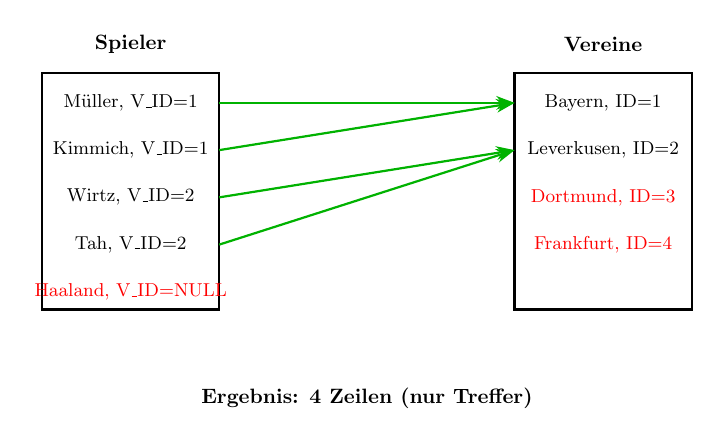
\begin{tikzpicture}[scale=0.75, every node/.style={scale=0.75}]
    % Spieler table
    \node[font=\bfseries] at (-4,3) {Spieler};
    \draw[thick] (-5.5,2.5) rectangle (-2.5,-1.5);
    \node[font=\small] at (-4,2) {Müller, V\_ID=1};
    \node[font=\small] at (-4,1.2) {Kimmich, V\_ID=1};
    \node[font=\small] at (-4,0.4) {Wirtz, V\_ID=2};
    \node[font=\small] at (-4,-0.4) {Tah, V\_ID=2};
    \node[font=\small, red] at (-4,-1.2) {Haaland, V\_ID=NULL};

    % Vereine table
    \node[font=\bfseries] at (4,3) {Vereine};
    \draw[thick] (2.5,2.5) rectangle (5.5,-1.5);
    \node[font=\small] at (4,2) {Bayern, ID=1};
    \node[font=\small] at (4,1.2) {Leverkusen, ID=2};
    \node[font=\small, red] at (4,0.4) {Dortmund, ID=3};
    \node[font=\small, red] at (4,-0.4) {Frankfurt, ID=4};

    % Arrows for matches
    \draw[-{Stealth}, thick, green!70!black] (-2.5,2) -- (2.5,2);
    \draw[-{Stealth}, thick, green!70!black] (-2.5,1.2) -- (2.5,2);
    \draw[-{Stealth}, thick, green!70!black] (-2.5,0.4) -- (2.5,1.2);
    \draw[-{Stealth}, thick, green!70!black] (-2.5,-0.4) -- (2.5,1.2);

    % Result
    \node[font=\bfseries] at (0,-3) {Ergebnis: 4 Zeilen (nur Treffer)};
\end{tikzpicture}
\end{center}
\end{frame}

\begin{frame}[fragile]{INNER JOIN: Alte vs. Neue Syntax}
\begin{columns}[T]
\column{0.5\textwidth}
\textbf{Explizite Syntax (SQL-92):}
\begin{lstlisting}
SELECT s.Name, v.Name
FROM Spieler s
INNER JOIN Vereine v
  ON s.Verein_ID = v.Verein_ID;
\end{lstlisting}

\vspace{0.5em}
{\color{green!70!black}\cmark} Klar erkennbar als JOIN\\
{\color{green!70!black}\cmark} Trennung von Join und Filter\\
{\color{green!70!black}\cmark} Empfohlener Standard

\column{0.5\textwidth}
\textbf{Implizite Syntax (alte Variante):}
\begin{lstlisting}
SELECT s.Name, v.Name
FROM Spieler s, Vereine v
WHERE s.Verein_ID = v.Verein_ID;
\end{lstlisting}

\vspace{0.5em}
{\color{red}\xmark} JOIN versteckt in WHERE\\
{\color{red}\xmark} Leicht vergessbar\\
{\color{red}\xmark} Wird kartesisches Produkt bei Fehler
\end{columns}

\vspace{1em}
\begin{alertblock}{Empfehlung}
Immer die \textbf{explizite} JOIN-Syntax verwenden! Klarer, sicherer, wartbarer.
\end{alertblock}
\end{frame}

\begin{frame}[fragile]{INNER JOIN: Mehrere Tabellen}
\textbf{Problem:} Alle Spiele mit Heim- und Gastverein-Namen?

\vspace{0.5em}
\begin{lstlisting}
SELECT
    sp.Datum,
    h.Name AS Heim,
    sp.Heim_Tore,
    sp.Gast_Tore,
    g.Name AS Gast
FROM Spiele sp
INNER JOIN Vereine h ON sp.Heim_ID = h.Verein_ID
INNER JOIN Vereine g ON sp.Gast_ID = g.Verein_ID;
\end{lstlisting}

\vspace{1em}
\textbf{Beachte:}
\begin{itemize}
    \item Zwei JOINs auf die \textbf{gleiche} Tabelle (Vereine)
    \item Unterschiedliche Aliase (h für Heim, g für Gast)
    \item JOINs werden von links nach rechts ausgeführt
\end{itemize}
\end{frame}

\begin{frame}[fragile]{Quiz: INNER JOIN verstehen}
\textbf{Gegeben:}
\begin{itemize}
    \item Spieler: 6 Zeilen (5 mit Verein, 1 mit NULL)
    \item Vereine: 4 Zeilen
\end{itemize}

\vspace{1em}
\textbf{Wie viele Zeilen liefert dieser Query?}
\begin{lstlisting}
SELECT s.Name, v.Name
FROM Spieler s
INNER JOIN Vereine v ON s.Verein_ID = v.Verein_ID;
\end{lstlisting}

\vspace{0.5em}
\begin{enumerate}
    \item[A)] 4 Zeilen (so viele wie Vereine)
    \item[B)] 5 Zeilen (Spieler mit Verein)
    \item[C)] 6 Zeilen (alle Spieler)
    \item[D)] 24 Zeilen (kartesisches Produkt)
\end{enumerate}

\pause
\vspace{0.5em}
\textbf{Antwort: B)} -- Nur Spieler mit passendem Verein (5 Treffer)
\end{frame}

% ===== Hands-on: INNER JOIN =====
{
\setbeamercolor{background canvas}{bg=IMSOrange!15}
\begin{frame}[plain]
\vfill
\begin{center}
{\Huge\color{IMSOrange} Hands-on}\\[1em]
{\Large INNER JOIN anwenden}\\[2em]
{\large\ttfamily marimo: 09-joins.py}\\[1em]
{\normalsize Aufgaben 9.1 -- 9.2}
\end{center}
\vfill
\end{frame}
}

% ===== PHASE 3: LEFT & RIGHT JOIN =====
\showagenda{3}

\begin{frame}{LEFT JOIN: Alle von links erhalten}
\begin{block}{Definition}
Der \textbf{LEFT JOIN} gibt \textbf{alle} Zeilen der linken Tabelle zurück, auch wenn kein Treffer in der rechten Tabelle existiert. Fehlende Werte werden mit \texttt{NULL} aufgefüllt.
\end{block}

\vspace{1em}
\begin{center}
\begin{tikzpicture}
    % Venn diagram - LEFT JOIN highlights entire left circle
    \fill[green!50] (-1,0) circle (1.5);  % Entire left circle highlighted
    \fill[IMSOrange!15] (1,0) circle (1.5);  % Right circle light
    \draw[thick, IMSBlue] (-1,0) circle (1.5) node[left=1.2cm, font=\bfseries] {Spieler};
    \draw[thick, IMSOrange] (1,0) circle (1.5) node[right=1.2cm, font=\bfseries] {Vereine};

    \node[font=\footnotesize] at (0,-2) {Alle Spieler, auch ohne Verein};
\end{tikzpicture}
\end{center}
\end{frame}

\begin{frame}[fragile]{LEFT JOIN: Syntax und Beispiel}
\begin{lstlisting}
SELECT s.Name, v.Name AS Verein
FROM Spieler s
LEFT JOIN Vereine v ON s.Verein_ID = v.Verein_ID;
\end{lstlisting}

\vspace{1em}
\textbf{Ergebnis:}
\begin{center}
\footnotesize
\begin{tabular}{|c|c|}
\hline
\rowcolor{IMSBlue!20}
\textbf{Name} & \textbf{Verein} \\
\hline
Müller & Bayern \\
\hline
Kimmich & Bayern \\
\hline
Wirtz & Leverkusen \\
\hline
Tah & Leverkusen \\
\hline
Neuer & Bayern \\
\hline
\rowcolor{yellow!20}
Haaland & NULL \\
\hline
\end{tabular}
\end{center}

\vspace{0.5em}
\textbf{Neu:} Haaland erscheint jetzt -- mit NULL für Verein!
\end{frame}

\begin{frame}[fragile]{LEFT JOIN: Fehlende Datensätze finden}
\textbf{Häufiges Muster:} ``Welche Spieler haben keinen Verein?''

\vspace{1em}
\begin{lstlisting}
SELECT s.Name
FROM Spieler s
LEFT JOIN Vereine v ON s.Verein_ID = v.Verein_ID
WHERE v.Verein_ID IS NULL;
\end{lstlisting}

\vspace{1em}
\textbf{Ergebnis:}
\begin{center}
\footnotesize
\begin{tabular}{|c|}
\hline
\rowcolor{IMSBlue!20}
\textbf{Name} \\
\hline
Haaland \\
\hline
\end{tabular}
\end{center}

\vspace{1em}
\begin{alertblock}{Wichtiges Muster}
\texttt{LEFT JOIN ... WHERE rechts.ID IS NULL} = ``Finde Zeilen ohne Treffer''
\end{alertblock}
\end{frame}

\begin{frame}{RIGHT JOIN: Alle von rechts erhalten}
\begin{block}{Definition}
Der \textbf{RIGHT JOIN} gibt \textbf{alle} Zeilen der rechten Tabelle zurück, auch wenn kein Treffer in der linken Tabelle existiert.
\end{block}

\vspace{1em}
\begin{center}
\begin{tikzpicture}
    % Venn diagram - RIGHT JOIN highlights entire right circle
    \fill[IMSBlue!15] (-1,0) circle (1.5);  % Left circle light
    \fill[green!50] (1,0) circle (1.5);  % Entire right circle highlighted
    \draw[thick, IMSBlue] (-1,0) circle (1.5) node[left=1.2cm, font=\bfseries] {Spieler};
    \draw[thick, IMSOrange] (1,0) circle (1.5) node[right=1.2cm, font=\bfseries] {Vereine};

    \node[font=\footnotesize] at (0,-2) {Alle Vereine, auch ohne Spieler};
\end{tikzpicture}
\end{center}

\vspace{0.5em}
\textbf{Hinweis:} RIGHT JOIN ist selten -- meist kann man die Tabellen tauschen und LEFT JOIN nutzen.
\end{frame}

\begin{frame}[fragile]{RIGHT JOIN: Beispiel}
\textbf{``Welche Vereine haben (k)eine Spieler?''}

\vspace{0.5em}
\begin{lstlisting}
SELECT v.Name AS Verein, COUNT(s.Spieler_ID) AS Anzahl
FROM Spieler s
RIGHT JOIN Vereine v ON s.Verein_ID = v.Verein_ID
GROUP BY v.Name;
\end{lstlisting}

\vspace{1em}
\textbf{Ergebnis:}
\begin{center}
\footnotesize
\begin{tabular}{|c|c|}
\hline
\rowcolor{IMSBlue!20}
\textbf{Verein} & \textbf{Anzahl} \\
\hline
Bayern & 3 \\
\hline
Leverkusen & 2 \\
\hline
\rowcolor{yellow!20}
Dortmund & 0 \\
\hline
\rowcolor{yellow!20}
Frankfurt & 0 \\
\hline
\end{tabular}
\end{center}

\vspace{0.5em}
\textbf{Neu:} Dortmund und Frankfurt erscheinen mit Anzahl 0!
\end{frame}

\begin{frame}{FULL OUTER JOIN: Alles erhalten}
\begin{block}{Definition}
Der \textbf{FULL OUTER JOIN} gibt \textbf{alle} Zeilen beider Tabellen zurück. Fehlende Werte werden mit \texttt{NULL} aufgefüllt.
\end{block}

\vspace{1em}
\begin{center}
\begin{tikzpicture}
    % Venn diagram - FULL OUTER JOIN highlights both circles
    \fill[green!50] (-1,0) circle (1.5);  % Entire left circle highlighted
    \fill[green!50] (1,0) circle (1.5);  % Entire right circle highlighted
    \draw[thick, IMSBlue] (-1,0) circle (1.5) node[left=1.2cm, font=\bfseries] {Spieler};
    \draw[thick, IMSOrange] (1,0) circle (1.5) node[right=1.2cm, font=\bfseries] {Vereine};

    \node[font=\footnotesize] at (0,-2) {Alle Spieler + Alle Vereine};
\end{tikzpicture}
\end{center}

\vspace{0.5em}
\begin{alertblock}{Hinweis zur Kompatibilität}
FULL OUTER JOIN wird von DuckDB und PostgreSQL unterstützt. SQLite unterstützt ihn \textbf{nicht} direkt (Workaround: LEFT + RIGHT JOIN mit UNION).
\end{alertblock}
\end{frame}

\begin{frame}{JOIN-Typen: Zusammenfassung}
\begin{center}
\footnotesize
\begin{tabular}{|l|p{5cm}|c|c|}
\hline
\rowcolor{IMSBlue!20}
\textbf{JOIN-Typ} & \textbf{Beschreibung} & \textbf{Ohne Match links} & \textbf{Ohne Match rechts} \\
\hline
INNER JOIN & Nur Treffer & \xmark{} ausgeschlossen & \xmark{} ausgeschlossen \\
\hline
LEFT JOIN & Alle links, Treffer rechts & \cmark{} mit NULL & \xmark{} ausgeschlossen \\
\hline
RIGHT JOIN & Treffer links, alle rechts & \xmark{} ausgeschlossen & \cmark{} mit NULL \\
\hline
FULL OUTER & Alle beider Seiten & \cmark{} mit NULL & \cmark{} mit NULL \\
\hline
\end{tabular}
\end{center}

\vspace{1em}
\textbf{Praxis-Empfehlung:}
\begin{itemize}
    \item \textbf{INNER JOIN}: Standard, wenn nur vollständige Daten benötigt
    \item \textbf{LEFT JOIN}: Wenn die linke Tabelle komplett bleiben soll
    \item \textbf{RIGHT JOIN}: Selten -- lieber Tabellen tauschen und LEFT nutzen
    \item \textbf{FULL OUTER}: Selten -- bei Datenabgleich/-vergleich
\end{itemize}
\end{frame}

\begin{frame}[fragile]{Quiz: Welcher JOIN?}
\textbf{Anforderung:} ``Liste alle Vereine mit der Anzahl ihrer Spieler. Vereine ohne Spieler sollen mit 0 erscheinen.''

\vspace{1em}
Welcher JOIN ist korrekt?

\vspace{0.5em}
\begin{enumerate}
    \item[A)] \texttt{Vereine INNER JOIN Spieler}
    \item[B)] \texttt{Spieler LEFT JOIN Vereine}
    \item[C)] \texttt{Vereine LEFT JOIN Spieler}
    \item[D)] \texttt{Spieler INNER JOIN Vereine}
\end{enumerate}

\pause
\vspace{0.5em}
\textbf{Antwort: C)} -- Alle Vereine (links) erhalten, auch ohne Spieler-Treffer.

\vspace{0.5em}
\begin{lstlisting}
SELECT v.Name, COUNT(s.Spieler_ID) AS Anzahl
FROM Vereine v
LEFT JOIN Spieler s ON v.Verein_ID = s.Verein_ID
GROUP BY v.Name;
\end{lstlisting}
\end{frame}

% ===== Hands-on + PAUSE =====
{
\setbeamercolor{background canvas}{bg=IMSOrange!15}
\begin{frame}[plain]
\vfill
\begin{center}
{\Huge\color{IMSOrange} Hands-on}\\[1em]
{\Large LEFT JOIN und fehlende Daten finden}\\[2em]
{\large\ttfamily marimo: 09-joins.py}\\[1em]
{\normalsize Aufgaben 9.3 -- 9.4}
\end{center}
\vfill
\end{frame}
}

% ===== PAUSE =====
\begin{frame}[plain]
\vfill
\begin{center}
{\Huge Pause}\\[1em]
{\LARGE 15 Minuten}\\[0.5em]
{\large Kaffee holen!}
\end{center}
\vfill
\end{frame}

% ===== PHASE 4: Self-Joins =====
\showagenda{4}

\begin{frame}{Self-Join: Eine Tabelle mit sich selbst}
\begin{block}{Definition}
Ein \textbf{Self-Join} verknüpft eine Tabelle mit \textbf{sich selbst}. Dabei werden Aliase verwendet, um die beiden ``Kopien'' zu unterscheiden.
\end{block}

\vspace{1em}
\textbf{Typische Anwendungsfälle:}
\begin{itemize}
    \item Hierarchien (Mitarbeiter $\rightarrow$ Vorgesetzter)
    \item Vergleiche innerhalb einer Tabelle
    \item Beziehungen zwischen Elementen der gleichen Menge
    \item Graphen und Netzwerke
\end{itemize}

\vspace{1em}
\begin{center}
\begin{tikzpicture}
    \node[roadmapbox, minimum width=3cm] (t1) at (0,0) {Tabelle T (als A)};
    \node[roadmapbox, minimum width=3cm] (t2) at (5,0) {Tabelle T (als B)};
    \draw[roadmaparrow] (t1) -- (t2) node[midway, above] {JOIN};
\end{tikzpicture}
\end{center}
\end{frame}

\begin{frame}[fragile]{Self-Join: Beispiel Hierarchie}
\textbf{Szenario:} Mitarbeiter mit ihren Vorgesetzten

\vspace{0.5em}
\begin{center}
\footnotesize
\begin{tabular}{|c|c|c|}
\hline
\rowcolor{IMSBlue!20}
\textbf{MA\_ID} & \textbf{Name} & \textbf{Chef\_ID} \\
\hline
1 & Müller (CEO) & NULL \\
\hline
2 & Schmidt & 1 \\
\hline
3 & Weber & 1 \\
\hline
4 & Fischer & 2 \\
\hline
5 & Bauer & 2 \\
\hline
\end{tabular}
\end{center}

\vspace{0.5em}
\begin{lstlisting}
SELECT m.Name AS Mitarbeiter, c.Name AS Chef
FROM Mitarbeiter m
LEFT JOIN Mitarbeiter c ON m.Chef_ID = c.MA_ID;
\end{lstlisting}

\vspace{0.5em}
\textbf{Ergebnis:} Schmidt $\rightarrow$ Müller, Weber $\rightarrow$ Müller, Fischer $\rightarrow$ Schmidt, ...
\end{frame}

\begin{frame}[fragile]{Self-Join: Spiele (Heim vs. Gast)}
\textbf{Problem:} Spiele mit Heim- und Gastnamen (beide aus Vereine)

\vspace{0.5em}
\begin{lstlisting}
SELECT
    sp.Datum,
    h.Name AS Heim,
    sp.Heim_Tore || ':' || sp.Gast_Tore AS Ergebnis,
    g.Name AS Gast
FROM Spiele sp
JOIN Vereine h ON sp.Heim_ID = h.Verein_ID
JOIN Vereine g ON sp.Gast_ID = g.Verein_ID;
\end{lstlisting}

\vspace{1em}
\textbf{Ergebnis:}
\begin{center}
\footnotesize
\begin{tabular}{|c|c|c|c|}
\hline
\rowcolor{IMSBlue!20}
\textbf{Datum} & \textbf{Heim} & \textbf{Ergebnis} & \textbf{Gast} \\
\hline
2026-03-15 & Bayern & 2:1 & Dortmund \\
\hline
2026-03-16 & Leverkusen & 3:0 & Frankfurt \\
\hline
\end{tabular}
\end{center}

\vspace{0.5em}
\textbf{Beachte:} Zwei JOINs auf Vereine mit unterschiedlichen Aliasen (h, g)!
\end{frame}

\begin{frame}[fragile]{Self-Join: Spieler im gleichen Verein}
\textbf{Problem:} Welche Spieler spielen im gleichen Verein?

\vspace{0.5em}
\begin{lstlisting}
SELECT
    s1.Name AS Spieler1,
    s2.Name AS Spieler2,
    v.Name AS Verein
FROM Spieler s1
JOIN Spieler s2 ON s1.Verein_ID = s2.Verein_ID
                AND s1.Spieler_ID < s2.Spieler_ID
JOIN Vereine v ON s1.Verein_ID = v.Verein_ID;
\end{lstlisting}

\vspace{0.5em}
\textbf{Ergebnis:}
\begin{center}
\footnotesize
\begin{tabular}{|c|c|c|}
\hline
\rowcolor{IMSBlue!20}
\textbf{Spieler1} & \textbf{Spieler2} & \textbf{Verein} \\
\hline
Müller & Kimmich & Bayern \\
\hline
Müller & Neuer & Bayern \\
\hline
Kimmich & Neuer & Bayern \\
\hline
Wirtz & Tah & Leverkusen \\
\hline
\end{tabular}
\end{center}

\vspace{0.3em}
\textbf{Wichtig:} \texttt{s1.ID < s2.ID} verhindert Duplikate und Selbst-Paare!
\end{frame}

% ===== PHASE 5: Exkurs Graphen =====
\showagenda{5}

\begin{frame}{Exkurs: Graphen als SQL-Tabellen}
\textbf{Motivation:} Self-Joins ermöglichen einfache Graph-Operationen!

\vspace{1em}
\begin{columns}[T]
\column{0.5\textwidth}
\textbf{Graph als Edge-List:}
\begin{center}
\begin{tikzpicture}[scale=0.9]
    \node[graphnode] (a) at (0,2) {A};
    \node[graphnode] (b) at (2,2) {B};
    \node[graphnode] (c) at (3,0) {C};
    \node[graphnode] (d) at (1,0) {D};
    \node[graphnode] (e) at (-1,0) {E};

    \draw[graphedge] (a) -- (b);
    \draw[graphedge] (a) -- (d);
    \draw[graphedge] (b) -- (c);
    \draw[graphedge] (b) -- (d);
    \draw[graphedge] (d) -- (e);
\end{tikzpicture}
\end{center}

\column{0.5\textwidth}
\textbf{Als Tabelle:}
\begin{center}
\footnotesize
\begin{tabular}{|c|c|}
\hline
\rowcolor{IMSBlue!20}
\textbf{von} & \textbf{nach} \\
\hline
A & B \\
\hline
A & D \\
\hline
B & C \\
\hline
B & D \\
\hline
D & E \\
\hline
\end{tabular}
\end{center}
\end{columns}

\vspace{1em}
\textbf{Idee:} Jede Kante ist eine Zeile mit (Quelle, Ziel).
\end{frame}

\begin{frame}[fragile]{Soziales Netzwerk als Graph}
\textbf{Beispiel:} Freundschaftsbeziehungen

\vspace{0.5em}
\begin{lstlisting}
CREATE TABLE friendships (
    person_a TEXT,
    person_b TEXT
);
\end{lstlisting}

\vspace{0.5em}
\begin{center}
\footnotesize
\begin{tabular}{|c|c|}
\hline
\rowcolor{IMSBlue!20}
\textbf{person\_a} & \textbf{person\_b} \\
\hline
Alice & Bob \\
\hline
Alice & Carol \\
\hline
Bob & Dave \\
\hline
Carol & Dave \\
\hline
Carol & Eve \\
\hline
\end{tabular}
\end{center}

\vspace{0.5em}
\textbf{Frage:} Wer sind die ``Freunde von Freunden'' von Alice?
\end{frame}

\begin{frame}[fragile]{Self-Join: Freunde von Freunden}
\textbf{2-Hop-Pfad mit Self-Join:}

\vspace{0.5em}
\begin{lstlisting}
SELECT DISTINCT f2.person_b AS friend_of_friend
FROM friendships f1
JOIN friendships f2 ON f1.person_b = f2.person_a
WHERE f1.person_a = 'Alice'
  AND f2.person_b <> 'Alice';
\end{lstlisting}

\vspace{1em}
\begin{center}
\begin{tikzpicture}[scale=0.9]
    \node[graphnode, fill=IMSOrange!40] (alice) at (0,0) {Alice};
    \node[graphnode] (bob) at (2,1) {Bob};
    \node[graphnode] (carol) at (2,-1) {Carol};
    \node[graphnode, fill=green!30] (dave) at (4,0) {Dave};
    \node[graphnode, fill=green!30] (eve) at (4,-1.5) {Eve};

    \draw[graphedge, IMSOrange, thick] (alice) -- (bob) node[midway, above, font=\tiny] {f1};
    \draw[graphedge, IMSOrange, thick] (alice) -- (carol) node[midway, below, font=\tiny] {f1};
    \draw[graphedge, green!70!black, thick] (bob) -- (dave) node[midway, above, font=\tiny] {f2};
    \draw[graphedge, green!70!black, thick] (carol) -- (dave) node[midway, above, font=\tiny] {f2};
    \draw[graphedge, green!70!black, thick] (carol) -- (eve) node[midway, below, font=\tiny] {f2};
\end{tikzpicture}
\end{center}

\vspace{0.3em}
\textbf{Ergebnis:} Dave, Eve (Freunde von Freunden)
\end{frame}

\begin{frame}{Was SQL nicht kann: Graph-Limitierungen}
\textbf{Grenzen von SQL bei Graphen:}

\vspace{1em}
\begin{columns}[T]
\column{0.5\textwidth}
\textbf{Geht mit SQL:}
\begin{itemize}
    \item Direkte Nachbarn (1 Hop)
    \item 2-Hop-Pfade (Self-Join)
    \item N-Hop-Pfade (N JOINs)
    \item Zyklen fester Länge
\end{itemize}

\column{0.5\textwidth}
\textbf{Geht NICHT (oder schwer):}
\begin{itemize}
    \item Kürzester Pfad beliebiger Länge
    \item PageRank
    \item Zusammenhangskomponenten
    \item Transitive Hülle (alle Pfade)
\end{itemize}
\end{columns}

\vspace{1em}
\begin{alertblock}{Fazit}
Für komplexe Graph-Analysen: Spezialisierte Tools nutzen!
\begin{itemize}
    \item \textbf{Python:} NetworkX
    \item \textbf{Datenbanken:} Neo4j, Amazon Neptune
    \item \textbf{Big Data:} Apache Spark GraphX
\end{itemize}
\end{alertblock}
\end{frame}

\begin{frame}{Rekursive CTEs: Ein Ausblick}
\textbf{SQL kann mehr mit ``Recursive CTE'':}

\vspace{1em}
\begin{center}
\begin{tikzpicture}[scale=0.8]
    \node[roadmapbox] (start) at (0,0) {Startwert};
    \node[roadmapbox, fill=IMSOrange!20] (iter) at (4,0) {Iteration};
    \node[roadmapbox, fill=green!20] (end) at (8,0) {Ergebnis};

    \draw[roadmaparrow] (start) -- (iter) node[midway, above, font=\footnotesize] {UNION};
    \draw[roadmaparrow] (iter) -- (end);
    \draw[roadmaparrow, bend right=40] (iter) to node[below, font=\footnotesize] {Rekursion} (iter);
\end{tikzpicture}
\end{center}

\vspace{1em}
\textbf{Damit möglich:}
\begin{itemize}
    \item Transitive Hülle (alle erreichbaren Knoten)
    \item Hierarchie-Traversierung beliebiger Tiefe
    \item Pfade in Graphen
\end{itemize}

\vspace{0.5em}
\textbf{Hinweis:} Wird in Session 10 (Subqueries \& CTEs) vertieft.
\end{frame}

% ===== PHASE 6: Join-Performance =====
\showagenda{6}

\begin{frame}{Join-Performance: Warum es wichtig ist}
\textbf{JOINs können teuer sein:}

\vspace{1em}
\begin{center}
\begin{tikzpicture}
    \node[roadmapbox, minimum width=2.5cm] (t1) at (0,0) {1.000 Zeilen};
    \node[roadmapbox, minimum width=2.5cm] (t2) at (4,0) {1.000 Zeilen};
    \node[roadmapbox, minimum width=3cm, fill=red!20] (result) at (8,0) {1.000.000?};

    \draw[roadmaparrow] (t1) -- (t2) node[midway, above] {JOIN};
    \draw[roadmaparrow] (t2) -- (result) node[midway, above] {ohne Optimierung};
\end{tikzpicture}
\end{center}

\vspace{1em}
\textbf{Kartesisches Produkt:}
\begin{itemize}
    \item Ohne Bedingung: $n \times m$ Kombinationen
    \item 1.000 $\times$ 1.000 = 1.000.000 potentielle Paare
    \item Datenbankoptimizer reduziert das -- aber nur mit Index!
\end{itemize}
\end{frame}

\begin{frame}{Join-Algorithmen: Überblick}
\textbf{Wie die Datenbank JOINs ausführt:}

\vspace{1em}
\begin{center}
\begin{tabular}{|l|p{4cm}|p{4cm}|}
\hline
\rowcolor{IMSBlue!20}
\textbf{Algorithmus} & \textbf{Funktionsweise} & \textbf{Wann gut?} \\
\hline
\textbf{Nested Loop} & Für jede Zeile links: durchsuche rechts & Kleine Tabellen, Index rechts \\
\hline
\textbf{Hash Join} & Hash-Tabelle bauen, dann matchen & Große Tabellen, kein Index \\
\hline
\textbf{Merge Join} & Beide sortiert, parallel durchlaufen & Bereits sortierte Daten \\
\hline
\end{tabular}
\end{center}

\vspace{1em}
\textbf{Der Optimizer wählt automatisch!}

Aber: Wir können helfen durch:
\begin{itemize}
    \item Indizes auf Join-Spalten
    \item Sinnvolle Join-Reihenfolge
    \item Vermeidung von Funktionen auf Join-Spalten
\end{itemize}
\end{frame}

\begin{frame}{Indizes für JOIN-Performance}
\begin{block}{Regel}
Join-Spalten sollten \textbf{indiziert} sein -- besonders die Fremdschlüssel!
\end{block}

\vspace{1em}
\textbf{Ohne Index:}
\begin{itemize}
    \item Datenbank muss \textbf{alle} Zeilen durchsuchen
    \item Bei großen Tabellen: sehr langsam
\end{itemize}

\vspace{0.5em}
\textbf{Mit Index:}
\begin{itemize}
    \item Direkter Zugriff auf passende Zeilen
    \item Logarithmische statt linearer Suche
\end{itemize}

\vspace{1em}
\begin{center}
\begin{tikzpicture}
    \node[roadmapbox, fill=red!20] at (0,0) {1.000.000 Zeilen scannen};
    \node[roadmapbox, fill=green!20] at (6,0) {20 Index-Lookups};
    \draw[roadmaparrow] (2.5,0) -- (3.5,0) node[midway, above, font=\small] {Index};
\end{tikzpicture}
\end{center}
\end{frame}

\begin{frame}[fragile]{EXPLAIN: Query-Plan analysieren}
\textbf{Mit EXPLAIN sehen, was die Datenbank plant:}

\vspace{0.5em}
\begin{lstlisting}
EXPLAIN
SELECT s.Name, v.Name
FROM Spieler s
JOIN Vereine v ON s.Verein_ID = v.Verein_ID;
\end{lstlisting}

\vspace{1em}
\textbf{Typische Operatoren im Query-Plan:}
\begin{itemize}
    \item \texttt{SCAN / SEQ\_SCAN}: Alle Zeilen durchlaufen (langsam bei großen Tabellen)
    \item \texttt{INDEX\_SCAN}: Index-Lookup (schnell)
    \item \texttt{HASH\_JOIN}: Hash-basierter Join
    \item \texttt{MERGE\_JOIN}: Sortier-basierter Join
\end{itemize}

\vspace{0.5em}
\small\textit{Hinweis: Die genaue Ausgabe variiert je nach Datenbank (DuckDB, PostgreSQL, SQLite, ...)}
\end{frame}

\begin{frame}{Best Practices: JOINs optimieren}
\textbf{1. Indizes erstellen:}
\begin{itemize}
    \item Alle Fremdschlüssel indizieren
    \item Häufig gefilterte Spalten indizieren
\end{itemize}

\vspace{0.5em}
\textbf{2. Früh filtern:}
\begin{itemize}
    \item WHERE-Bedingungen so früh wie möglich
    \item Weniger Zeilen im JOIN = schneller
\end{itemize}

\vspace{0.5em}
\textbf{3. Nur benötigte Spalten:}
\begin{itemize}
    \item \texttt{SELECT *} vermeiden
    \item Explizit nur benötigte Spalten auswählen
\end{itemize}

\vspace{0.5em}
\textbf{4. Join-Reihenfolge beachten:}
\begin{itemize}
    \item Kleine Tabelle zuerst (bei manchen Datenbanken)
    \item Optimizer macht das meist automatisch
\end{itemize}
\end{frame}

\begin{frame}{CROSS JOIN: Das kartesische Produkt}
\begin{block}{Definition}
Ein \textbf{CROSS JOIN} erzeugt alle möglichen Kombinationen -- \textbf{ohne} Bedingung.
\end{block}

\vspace{1em}
\textbf{Selten gewollt, aber nützlich für:}
\begin{itemize}
    \item Kalender/Zeitreihen generieren
    \item Alle Kombinationen erzeugen
    \item Test-Datensätze erstellen
\end{itemize}

\vspace{1em}
\begin{center}
\begin{tabular}{|c|c|c|}
\hline
\rowcolor{IMSBlue!20}
\textbf{Links (3)} & \textbf{Rechts (4)} & \textbf{CROSS (12)} \\
\hline
A & 1 & A-1, A-2, A-3, A-4 \\
B & 2 & B-1, B-2, B-3, B-4 \\
C & 3 & C-1, C-2, C-3, C-4 \\
 & 4 & \\
\hline
\end{tabular}
\end{center}
\end{frame}

\begin{frame}[fragile]{NATURAL JOIN und USING}
\textbf{Kurzschreibweisen (mit Vorsicht zu genießen):}

\vspace{1em}
\textbf{USING -- wenn Spaltenname identisch:}
\begin{lstlisting}
SELECT * FROM Spieler
JOIN Vereine USING (Verein_ID);
\end{lstlisting}

\vspace{0.5em}
{\color{green!70!black}\cmark} Kurz und lesbar bei gleichnamigen Spalten

\vspace{1em}
\textbf{NATURAL JOIN -- automatisch nach gleichen Namen:}
\begin{lstlisting}
SELECT * FROM Spieler
NATURAL JOIN Vereine;
\end{lstlisting}

\vspace{0.5em}
{\color{red}\xmark} Gefährlich! Joined auf \textbf{alle} gleichnamigen Spalten -- auch unbeabsichtigt!

\vspace{1em}
\begin{alertblock}{Empfehlung}
USING ist akzeptabel. NATURAL JOIN vermeiden -- zu implizit, fehleranfällig.
\end{alertblock}
\end{frame}

% ===== Hands-on =====
{
\setbeamercolor{background canvas}{bg=IMSOrange!15}
\begin{frame}[plain]
\vfill
\begin{center}
{\Huge\color{IMSOrange} Hands-on}\\[1em]
{\Large Self-Joins und Performance}\\[2em]
{\large\ttfamily marimo: 09-joins.py}\\[1em]
{\normalsize Aufgaben 9.5 -- 9.7}
\end{center}
\vfill
\end{frame}
}

% ===== PHASE 7: Zusammenfassung =====
\showagenda{7}

\begin{frame}{Zusammenfassung: JOIN-Typen}
\begin{center}
\begin{tikzpicture}[scale=0.7]
    % INNER
    \begin{scope}[shift={(-4.5,1.5)}]
        \draw[thick, IMSBlue, fill=IMSBlue!10] (0,0) circle (0.8);
        \draw[thick, IMSOrange, fill=IMSOrange!10] (0.7,0) circle (0.8);
        \begin{scope}
            \clip (0,0) circle (0.8);
            \fill[green!40] (0.7,0) circle (0.8);
        \end{scope}
        \node[font=\footnotesize\bfseries] at (0.35,-1.3) {INNER};
    \end{scope}

    % LEFT
    \begin{scope}[shift={(-1.5,1.5)}]
        \draw[thick, IMSBlue, fill=IMSBlue!30] (0,0) circle (0.8);
        \draw[thick, IMSOrange, fill=IMSOrange!10] (0.7,0) circle (0.8);
        \begin{scope}
            \clip (0,0) circle (0.8);
            \fill[green!40] (0.7,0) circle (0.8);
        \end{scope}
        \node[font=\footnotesize\bfseries] at (0.35,-1.3) {LEFT};
    \end{scope}

    % RIGHT
    \begin{scope}[shift={(1.5,1.5)}]
        \draw[thick, IMSBlue, fill=IMSBlue!10] (0,0) circle (0.8);
        \draw[thick, IMSOrange, fill=IMSOrange!30] (0.7,0) circle (0.8);
        \begin{scope}
            \clip (0,0) circle (0.8);
            \fill[green!40] (0.7,0) circle (0.8);
        \end{scope}
        \node[font=\footnotesize\bfseries] at (0.35,-1.3) {RIGHT};
    \end{scope}

    % FULL
    \begin{scope}[shift={(4.5,1.5)}]
        \draw[thick, IMSBlue, fill=IMSBlue!30] (0,0) circle (0.8);
        \draw[thick, IMSOrange, fill=IMSOrange!30] (0.7,0) circle (0.8);
        \begin{scope}
            \clip (0,0) circle (0.8);
            \fill[green!40] (0.7,0) circle (0.8);
        \end{scope}
        \node[font=\footnotesize\bfseries] at (0.35,-1.3) {FULL OUTER};
    \end{scope}
\end{tikzpicture}
\end{center}

\vspace{0.5em}
\begin{itemize}
    \item \textbf{INNER JOIN}: Nur Treffer beider Seiten
    \item \textbf{LEFT JOIN}: Alle links + Treffer (NULL wenn kein Match)
    \item \textbf{RIGHT JOIN}: Treffer + Alle rechts (selten benötigt)
    \item \textbf{FULL OUTER}: Alle beider Seiten (nicht in SQLite)
\end{itemize}
\end{frame}

\begin{frame}{Zusammenfassung: Wichtige Muster}
\textbf{1. Fehlende Daten finden:}
\begin{itemize}
    \item \texttt{LEFT JOIN ... WHERE rechts.ID IS NULL}
    \item ``Spieler ohne Verein'', ``Vereine ohne Spieler''
\end{itemize}

\vspace{0.5em}
\textbf{2. Self-Join für interne Beziehungen:}
\begin{itemize}
    \item Gleiche Tabelle mit verschiedenen Aliasen
    \item Hierarchien, Vergleiche, Graphen
\end{itemize}

\vspace{0.5em}
\textbf{3. Mehrere JOINs verketten:}
\begin{itemize}
    \item \texttt{FROM A JOIN B JOIN C}
    \item Spiele mit Heim- und Gast-Vereinsnamen
\end{itemize}

\vspace{0.5em}
\textbf{4. Performance beachten:}
\begin{itemize}
    \item Indizes auf Fremdschlüsseln
    \item EXPLAIN zur Analyse
\end{itemize}
\end{frame}

\begin{frame}{Cheat Sheet: JOIN-Syntax}
\begin{center}
\footnotesize
\begin{tabular}{|l|p{8cm}|}
\hline
\rowcolor{IMSBlue!20}
\textbf{Muster} & \textbf{SQL-Syntax} \\
\hline
INNER JOIN & \texttt{FROM A INNER JOIN B ON A.id = B.a\_id} \\
\hline
LEFT JOIN & \texttt{FROM A LEFT JOIN B ON A.id = B.a\_id} \\
\hline
RIGHT JOIN & \texttt{FROM A RIGHT JOIN B ON A.id = B.a\_id} \\
\hline
Self-Join & \texttt{FROM T t1 JOIN T t2 ON t1.x = t2.y} \\
\hline
Mehrfach-Join & \texttt{FROM A JOIN B ON ... JOIN C ON ...} \\
\hline
Fehlende finden & \texttt{LEFT JOIN ... WHERE B.id IS NULL} \\
\hline
USING & \texttt{FROM A JOIN B USING (gemeinsame\_spalte)} \\
\hline
\end{tabular}
\end{center}

\vspace{1em}
\textbf{Merksatz:}
\begin{quote}
``Die linke Tabelle bestimmt die Grundmenge bei LEFT JOIN -- alle ihre Zeilen bleiben erhalten.''
\end{quote}
\end{frame}

\begin{frame}{Häufige Fehler vermeiden}
\begin{columns}[T]
\column{0.5\textwidth}
\textbf{\xmark{} Fehler:}
\begin{itemize}
    \item JOIN ohne ON-Bedingung\\
    $\rightarrow$ Kartesisches Produkt!
    \item Falsche Spalte im JOIN\\
    $\rightarrow$ Unerwartete Ergebnisse
    \item LEFT statt INNER verwechselt\\
    $\rightarrow$ NULL-Werte unerwartet
    \item Fehlende Aliase bei Self-Join\\
    $\rightarrow$ Syntax-Fehler
\end{itemize}

\column{0.5\textwidth}
\textbf{\cmark{} Best Practices:}
\begin{itemize}
    \item Immer explizite ON-Klausel
    \item Aliase bei mehrdeutigen Spaltennamen
    \item Tabellenname.Spalte bei JOINs
    \item EXPLAIN bei langsamen Queries
    \item Indizes auf FK-Spalten
\end{itemize}
\end{columns}

\vspace{1em}
\begin{alertblock}{Tipp}
Bei unerwarteten Ergebnissen: Erst ohne WHERE prüfen, dann Filter hinzufügen.
\end{alertblock}
\end{frame}

\begin{frame}{Ausblick: Nächste Vorlesung}
\textbf{Vorlesung 10: Subqueries, Views \& Transaktionen}

\vspace{1em}
\begin{itemize}
    \item Subqueries: Abfragen in Abfragen
    \item Common Table Expressions (WITH)
    \item Views: Virtuelle Tabellen
    \item ACID und Transaktionen
\end{itemize}

\vspace{2em}
\begin{center}
\begin{tikzpicture}
    \node[roadmapbox] (join) at (0,0) {JOINs verstanden};
    \node[roadmapbox, fill=IMSOrange!20, draw=IMSOrange] (sub) at (6,0) {Subqueries \& CTEs};
    \draw[roadmaparrow] (join) -- (sub) node[midway, above] {komplexere Strukturen};
\end{tikzpicture}
\end{center}

\vspace{1em}
\textbf{Mit JOINs und Subqueries sind fast alle SQL-Abfragen möglich!}
\end{frame}

\begin{frame}[plain]
\vfill
\begin{center}
{\Huge Fragen?}\\[2em]
{\large christoph.flath@uni-wuerzburg.de}
\end{center}
\vfill
\end{frame}

\end{document}
